%!TeX root=../houndtop.tex
\chapter{The Curse of the Baskervilles}
\lettrine[ante=`,lines=1]{I}{} have in my pocket a manuscript,' said Dr James Mortimer.

»I observed it as you entered the room,« said Holmes.

»It is an old manuscript.«

»Early eighteenth century, unless it is a forgery.«

»How can you say that, sir?«

»You have presented an inch or two of it to my examination all the time that you have been talking. It would be a poor expert who could not give the date of a document within a decade or so. You may possibly have read my little monograph upon the subject. I put that at 1730.«

»The exact date is 1742.« Dr Mortimer drew it from his breast-pocket. »This family paper was committed to my care by Sir Charles Baskerville, whose sudden and tragic death some three months ago created so much excitement in Devonshire. I may say that I was his personal friend as well as his medical attendant. He was a strong-minded man, sir, shrewd, practical, and as unimaginative as I am myself. Yet he took this document very seriously, and his mind was prepared for just such an end as did eventually overtake him.«

Holmes stretched out his hand for the manuscript and flattened it upon his knee.

»You will observe, Watson, the alternative use of the long \textit{s} and the short. It is one of several indications which enabled me to fix the date.«

I looked over his shoulder at the yellow paper and the faded script. At the head was written: \oldfont Baskerville Hall\normalfont, and below in large, scrawling figures: \oldfont 1742. \normalfont

»It appears to be a statement of some sort.«

»Yes, it is a statement of a certain legend which runs in the Baskerville family.«

»But I understand that it is something more modern and practical upon which you wish to consult me?«

»Most modern. A most practical, pressing matter, which must be decided within twenty-four hours. But the manuscript is short and is intimately connected with the affair. With your permission I will read it to you.«

Holmes leaned back in his chair, placed his finger-tips together, and closed his eyes, with an air of resignation. Dr Mortimer turned the manuscript to the light and read in a high, cracking voice the following curious, old-world narrative:— 

\noindent\hfil\rule{0.5\textwidth}{.4pt}\hfil 

\oldfont
Of the origin of the Hound of the Baskervilles there have been many statements, yet as I come in a dire line from Hugo Baskerville, and as I had the story from my father, who also had it from his, I have set it down with all belief that it occurred even as is here set forth. And I would have you believe, my sons, that the same Juſtice which punishes sin may also moſt graciously forgive it, and that no ban is so heavy but that by prayer and repentance it may be removed. Learn then from this story not to fear the fruits of the paſt, but rather to be circumspe in the future, that those foul paßions whereby our family has suffered so grievously may not again be loosed to our undoing.

Know then that in the time of the Great Rebellion\footnote{First English Civil War, 1642-1646} (the hiſtory of which by the learned Lord Clarendon\footnote{\textit{The History of the Rebellion and Civil Wars in England}, by Edward Hyde, Lord Clarendon (1609-1674), first published in three volumes between 1702 and 1704.} I moſt earneſtly commend to your attention) this Manor of Baskerville was held by Hugo of that name, nor can it be gainsaid that he was a moſt wild, profane, and godleß man. This, in truth, his neighbours might have pardoned, seeing that saints have never flourished in those parts, but there was in him a certain wanton and cruel humour which made his name a byword through the Weſt. It chanced that this Hugo came to love (if, indeed, so dark a paßion may be known under so bright a name) the daughter of a yeoman who held lands near the Baskerville eſtate. But the young maiden, being discreet and of good repute, would ever avoid him, for she feared his evil name. So it came to paß that one Michaelmas\footnote{29\textsuperscript{th} September} this Hugo, with five or six of his idle and wicked companions, stole down upon the farm and carried off the maiden, her father and brothers being from home, as he well knew. When they had brought her to the Hall the maiden was placed in an upper chamber, while Hugo and his friends sat down to a long carouse, as was their nightly cuſtom. Now, the poor laß upſtairs was like to have her wits turned at the singing and shouting and terrible oaths which came up to her from below, for they say that the words used by Hugo Baskerville, when he was in wine, were such as might blaſt the man who said them. At laſt in the streß of her fear she did that which might have daunted the braveſt or moſt aive man, for by the aid of the growth of ivy which covered (and still covers) the south wall she came down from under the eaves, and so homeward acroß the moor, there being three leagues betwixt the Hall and her father's farm.

\begin{wrapfigure}{O}{0.5\textwidth}
\centering
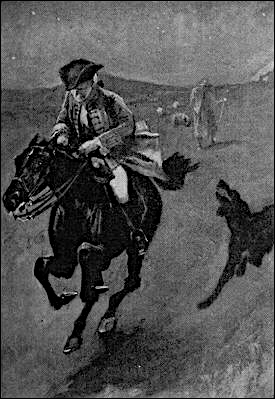
\includegraphics[width=0.5\textwidth]{02_blackmare}
\caption{Upon his black mare}
\end{wrapfigure}

It chanced that some little time later Hugo left his gueſts to carry food and drink\textemdash with other worse things, perchance\textemdash to his captive, and so found the cage empty and the bird escaped. Then, as it would seem, he became as one that hath a devil, for, rushing down the stairs into the dining-hall, he sprang upon the great table, flagons and trenchers flying before him, and he cried aloud before all the company that he would that very night render his body and soul to the Powers of Evil if he might but overtake the wench. And while the revellers stood aghaſt at the fury of the man, one more wicked or, it may be, more drunken than the reſt, cried out that they should put the hounds upon her. Whereat Hugo ran from the house, crying to his grooms that they should saddle his mare and unkennel the pack, and giving the hounds a kerchief of the maid's, he swung them to the line, and so off full cry in the moonlight over the moor.

Now, for some space the revellers stood agape, unable to underſtand all that had been done in such haſte. But anon their bemused wits awoke to the nature of the deed which was like to be done upon the moorlands. Everything was now in an uproar, some calling for their piſtols, some for their horses, and some for another flask of wine. But at length some sense came back to their crazed minds, and the whole of them, thirteen in number, took horse and started in pursuit. The moon shone clear above them, and they rode swiftly abreaſt, taking that course which the maid muſt needs have taken if she were to reach her own home.

They had gone a mile or two when they paßed one of the night shepherds upon the moorlands, and they cried to him to know if he had seen the hunt. And the man, as the story goes, was so crazed with fear that he could scarce speak, but at laſt he said that he had indeed seen the unhappy maiden, with the hounds upon her track. »But I have seen more than that,« said he, »for Hugo Baskerville paßed me upon his black mare, and there ran mute behind him such a hound of hell as God forbid should ever be at my heels.« So the drunken squires cursed the shepherd and rode onward. But soon their skins turned cold, for there came a galloping acroß the moor, and the black mare, dabbled with white froth, went paſt with trailing bridle and empty saddle. Then the revellers rode close together, for a great fear was on them, but they still followed over the moor, though each, had he been alone, would have been right glad to have turned his horse's head. Riding slowly in this fashion they came at laſt upon the hounds. These, though known for their valour and their breed, were whimpering in a cluſter at the head of a deep dip or goyal, as we call it, upon the moor, some slinking away and some, with starting hackles and staring eyes, gazing down the narrow valley before them.

The company had come to a halt, more sober men, as you may gueß, than when they started. The moſt of them would by no means advance, but three of them, the boldeſt, or it may be the moſt drunken, rode forward down the goyal. Now, it opened into a broad space in which stood two of those great stones, still to be seen there, which were set by certain forgotten peoples in the days of old. The moon was shining bright upon the clearing, and there in the centre lay the unhappy maid where she had fallen, dead of fear and of fatigue. But it was not the sight of her body, nor yet was it that of the body of Hugo Baskerville lying near her, which raised the hair upon the heads of these three daredevil royſterers, but it was that, standing over Hugo, and plucking at his throat, there stood a foul thing, a great, black beaſt, shaped like a hound, yet larger than any hound that ever mortal eye has reſted upon. And even as they looked the thing tore the throat out of Hugo Baskerville, on which, as it turned its blazing eyes and dripping jaws upon them, the three shrieked with fear and rode for dear life, still screaming, acroß the moor. One, it is said, died that very night of what he had seen, and the other twain were but broken men for the reſt of their days.

\begin{figure}[tbph]
\centering
\includegraphics[width=\linewidth]{02_unhappymaidbig}
\caption{There in the centre lay the unhappy maid}
\end{figure}

Such is the tale, my sons, of the coming of the hound which is said to have plagued the family so sorely ever since. If I have set it down it is because that which is clearly known hath leß terror than that which is but hinted at and gueßed. Nor can it be denied that many of the family have been unhappy in their deaths, which have been sudden, bloody, and myſterious. Yet may we shelter ourselves in the infinite goodneß of Providence, which would not forever punish the innocent beyond that third or fourth generation which is threatened in Holy Writ. To that Providence, my sons, I hereby commend you, and I counsel you by way of caution to forbear from croßing the moor in those dark hours when the powers of evil are exalted.

[This from Hugo Baskerville to his sons Rodger and John, with inſtruions that they say nothing thereof to their siſter Elizabeth.]
\normalfont
\noindent\hfil\rule{0.5\textwidth}{.4pt}\hfil 

When Dr Mortimer had finished reading this singular narrative he pushed his spectacles up on his forehead and stared across at Mr Sherlock Holmes. The latter yawned and tossed the end of his cigarette into the fire.

»Well?« said he.

»Do you not find it interesting?«

»To a collector of fairy tales.«

Dr Mortimer drew a folded newspaper out of his pocket.

»Now, Mr Holmes, we will give you something a little more recent. This is the \textit{Devon County Chronicle} of May 14\textsuperscript{th} of this year. It is a short account of the facts elicited at the death of Sir Charles Baskerville which occurred a few days before that date.«

My friend leaned a little forward and his expression became intent. Our visitor readjusted his glasses and began:— 

\noindent\hfil\rule{0.5\textwidth}{.4pt}\hfil 

\textsf{The recent sudden death of Sir Charles Baskerville, whose name has been mentioned as the probable Liberal candidate for Mid-Devon at the next election, has cast a gloom over the county. Though Sir Charles had resided at Baskerville Hall for a comparatively short period his amiability of character and extreme generosity had won the affection and respect of all who had been brought into contact with him. In these days of \emph{nouveaux riches} it is refreshing to find a case where the scion of an old county family which has fallen upon evil days is able to make his own fortune and to bring it back with him to restore the fallen grandeur of his line. Sir Charles, as is well known, made large sums of money in South African speculation. More wise than those who go on until the wheel turns against them, he realized his gains and returned to England with them. It is only two years since he took up his residence at Baskerville Hall, and it is common talk how large were those schemes of reconstruction and improvement which have been interrupted by his death. Being himself childless, it was his openly expressed desire that the whole country-side should, within his own lifetime, profit by his good fortune, and many will have personal reasons for bewailing his untimely end. His generous donations to local and county charities have been frequently chronicled in these columns.}

%\begin{wrapfigure}{O}{0.6\linewidth}
%\centering
%
\includegraphics[width=0.6\linewidth]{02_bodydiscovered}
%\caption{His body was discovered}
%\end{wrapfigure}

\textsf{The circumstances connected with the death of Sir Charles cannot be said to have been entirely cleared up by the inquest, but at least enough has been done to dispose of those rumours to which local superstition has given rise. There is no reason whatever to suspect foul play, or to imagine that death could be from any but natural causes. Sir Charles was a widower, and a man who may be said to have been in some ways of an eccentric habit of mind. In spite of his considerable wealth he was simple in his personal tastes, and his indoor servants at Baskerville Hall consisted of a married couple named Barrymore, the husband acting as butler and the wife as housekeeper. Their evidence, corroborated by that of several friends, tends to show that Sir Charles's health has for some time been impaired, and points especially to some affection of the heart, manifesting itself in changes of colour, breathlessness, and acute attacks of nervous depression. Dr James Mortimer, the friend and medical attendant of the deceased, has given evidence to the same effect.}

\textsf{The facts of the case are simple. Sir Charles Baskerville was in the habit every night before going to bed of walking down the famous Yew Alley of Baskerville Hall. The evidence of the Barrymores shows that this had been his custom. On the 4\textsuperscript{th} of May Sir Charles had declared his intention of starting next day for London, and had ordered Barrymore to prepare his luggage. That night he went out as usual for his nocturnal walk, in the course of which he was in the habit of smoking a cigar. He never returned. At twelve o'clock Barrymore, finding the hall door still open, became alarmed, and, lighting a lantern, went in search of his master. The day had been wet, and Sir Charles's footmarks were easily traced down the Alley. Half-way down this walk there is a gate which leads out on to the moor. There were indications that Sir Charles had stood for some little time here. He then proceeded down the Alley, and it was at the far end of it that his body was discovered. One fact which has not been explained is the statement of Barrymore that his master's footprints altered their character from the time that he passed the moor-gate, and that he appeared from thence onward to have been walking upon his toes. One Murphy, a gipsy horse-dealer, was on the moor at no great distance at the time, but he appears by his own confession to have been the worse for drink. He declares that he heard cries, but is unable to state from what direction they came. No signs of violence were to be discovered upon Sir Charles's person, and though the doctor's evidence pointed to an almost incredible facial distortion—so great that Dr Mortimer refused at first to believe that it was indeed his friend and patient who lay before him—it was explained that that is a symptom which is not unusual in cases of dyspnoea and death from cardiac exhaustion. This explanation was borne out by the post-mortem examination, which showed long-standing organic disease, and the coroner's jury returned a verdict in accordance with the medical evidence. It is well that this is so, for it is obviously of the utmost importance that Sir Charles's heir should settle at the Hall and continue the good work which has been so sadly interrupted. Had the prosaic finding of the coroner not finally put an end to the romantic stories which have been whispered in connection with the affair, it might have been difficult to find a tenant for Baskerville Hall. It is understood that the next of kin is Mr Henry Baskerville, if he be still alive, the son of Sir Charles Baskerville's younger brother. The young man when last heard of was in America, and inquiries are being instituted with a view to informing him of his good fortune.}

\noindent\hfil\rule{0.5\textwidth}{.4pt}\hfil 

Dr Mortimer refolded his paper and replaced it in his pocket.

»Those are the public facts, Mr Holmes, in connection with the death of Sir Charles Baskerville.«

»I must thank you,« said Sherlock Holmes, »for calling my attention to a case which certainly presents some features of interest. I had observed some newspaper comment at the time, but I was exceedingly preoccupied by that little affair of the Vatican cameos, and in my anxiety to oblige the Pope I lost touch with several interesting English cases. This article, you say, contains all the public facts?«

»It does.«

»Then let me have the private ones.« He leaned back, put his finger-tips together, and assumed his most impassive and judicial expression.

»In doing so,« said Dr Mortimer, who had begun to show signs of some strong emotion, »I am telling that which I have not confided to anyone. My motive for withholding it from the coroner's inquiry is that a man of science shrinks from placing himself in the public position of seeming to indorse a popular superstition. I had the further motive that Baskerville Hall, as the paper says, would certainly remain untenanted if anything were done to increase its already rather grim reputation. For both these reasons I thought that I was justified in telling rather less than I knew, since no practical good could result from it, but with you there is no reason why I should not be perfectly frank.«

»The moor is very sparsely inhabited, and those who live near each other are thrown very much together. For this reason I saw a good deal of Sir Charles Baskerville. With the exception of Mr Frankland, of Lafter Hall, and Mr Stapleton, the naturalist, there are no other men of education within many miles. Sir Charles was a retiring man, but the chance of his illness brought us together, and a community of interests in science kept us so. He had brought back much scientific information from South Africa, and many a charming evening we have spent together discussing the comparative anatomy of the Bushman\footnote{The San people of south-central Africa.} and the Hottentot\footnote{The Khoi people of the western Cape region of South Africa.}.«

»Within the last few months it became increasingly plain to me that Sir Charles's nervous system was strained to the breaking point. He had taken this legend which I have read you exceedingly to hear—so much so that, although he would walk in his own grounds, nothing would induce him to go out upon the moor at night. Incredible as it may appear to you, Mr Holmes, he was honestly convinced that a dreadful fate overhung his family, and certainly the records which he was able to give of his ancestors were not encouraging. The idea of some ghastly presence constantly haunted him, and on more than one occasion he has asked me whether I had on my medical journeys at night ever seen any strange creature or heard the baying of a hound. The latter question he put to me several times, and always with a voice which vibrated with excitement.«

\begin{figure}[tbhp]
\centering

\includegraphics[width=1.1\linewidth]{02_overshoulder}
\caption{I saw his eyes fix themselves over my shoulder}
\end{figure}

»I can well remember driving up to his house in the evening some three weeks before the fatal event. He chanced to be at his hall door. I had descended from my gig and was standing in front of him, when I saw his eyes fix themselves over my shoulder, and stare past me with an expression of the most dreadful horror. I whisked round and had just time to catch a glimpse of something which I took to be a large black calf passing at the head of the drive. So excited and alarmed was he that I was compelled to go down to the spot where the animal had been and look around for it. It was gone, however, and the incident appeared to make the worst impression upon his mind. I stayed with him all the evening, and it was on that occasion, to explain the emotion which he had shown, that he confided to my keeping that narrative which I read to you when first I came. I mention this small episode because it assumes some importance in view of the tragedy which followed, but I was convinced at the time that the matter was entirely trivial and that his excitement had no justification.«

»It was at my advice that Sir Charles was about to go to London. His heart was, I knew, affected, and the constant anxiety in which he lived, however chimerical the cause of it might be, was evidently having a serious effect upon his health. I thought that a few months among the distractions of town would send him back a new man. Mr Stapleton, a mutual friend who was much concerned at his state of health, was of the same opinion. At the last instant came this terrible catastrophe.«

»On the night of Sir Charles's death Barrymore the butler, who made the discovery, sent Perkins the groom on horseback to me, and as I was sitting up late I was able to reach Baskerville Hall within an hour of the event. I checked and corroborated all the facts which were mentioned at the inquest. I followed the footsteps down the Yew Alley, I saw the spot at the moor-gate where he seemed to have waited, I remarked the change in the shape of the prints after that point, I noted that there were no other footsteps save those of Barrymore on the soft gravel, and finally I carefully examined the body, which had not been touched until my arrival. Sir Charles lay on his face, his arms out, his fingers dug into the ground, and his features convulsed with some strong emotion to such an extent that I could hardly have sworn to his identity. There was certainly no physical injury of any kind. But one false statement was made by Barrymore at the inquest. He said that there were no traces upon the ground round the body. He did not observe any. But I did—some little distance off, but fresh and clear.«

»Footprints?«

»Footprints.«

»A man's or a woman's?«

Dr Mortimer looked strangely at us for an instant, and his voice sank almost to a whisper as he answered:— 

»Mr Holmes, they were the footprints of a gigantic hound!«
